\documentclass[a4paper]{article}
\setcounter{secnumdepth}{0}
%%%%%%%% CREATE DOCUMENT STRUCTURE %%%%%%%%
%% Language and font encodings
\usepackage[english]{babel}
\usepackage[utf8x]{inputenc}
\usepackage[T1]{fontenc}
%\usepackage{subfig}

%% Sets page size and margins
\usepackage[a4paper,top=2cm,bottom=2cm,left=2cm,right=2cm,marginparwidth=1.75cm]{geometry}

%% Useful packages
\usepackage{amsmath}
\usepackage{graphicx}
\usepackage[colorinlistoftodos]{todonotes}
\usepackage[colorlinks=true, allcolors=blue]{hyperref}
\usepackage{caption}
\usepackage{subcaption}
\usepackage{sectsty}
\usepackage{apacite}
\usepackage{float}
\usepackage{titling}
\usepackage{tabto} 
\usepackage{blindtext}
\usepackage[square,sort,comma,numbers]{natbib}
\usepackage[colorinlistoftodos]{todonotes}
\usepackage{xcolor}

\definecolor{darkgreen}{rgb}{0.0, 0.4, 0.0}

\usepackage{listings}
\usepackage{tabularx,booktabs}
\usepackage{xcolor}

\definecolor{codegreen}{rgb}{0,0.6,0}
\definecolor{codegray}{rgb}{0.5,0.5,0.5}
\definecolor{codepurple}{rgb}{0.58,0,0.82}
\definecolor{backcolour}{rgb}{0.95,0.95,0.92}

\lstdefinestyle{mystyle}{
    backgroundcolor=\color{backcolour},   
    commentstyle=\color{codegreen},
    keywordstyle=\color{magenta},
    numberstyle=\tiny\color{codegray},
    stringstyle=\color{codepurple},
    basicstyle=\ttfamily\footnotesize,
    breakatwhitespace=false,         
    breaklines=true,                 
    captionpos=b,                    
    keepspaces=true,                 
    numbers=left,                    
    numbersep=5pt,                  
    showspaces=false,                
    showstringspaces=false,
    showtabs=false,                  
    tabsize=2
}

\lstset{style=mystyle}
\definecolor{LightGray}{gray}{0.9}
\title{\textbf{EN2550 - Fundamentals of Image Processing and Machine Vision}\\
Assignment 01}
\author{Tharindu O.K.D.\\19062R}


\begin{document}

\maketitle

GitHub Repository https://github.com/dakshinatharindu/Image-Processing/tree/main/Assignment-01
\section*{Question 01}

The intensity transformation is a way of mapping the intensity values of
 an image according to a given function. As shown in the below code, we
  can use the OpenCV LookUpTable (cv.LUT) method to map the intensity values.


\begin{lstlisting}[language=python, caption=Intensity Iransformation, label=q1c]
array_1 = np.array([ i for i in range(0,51)])
array_2 = np.array([ (155 / 100) * (i - 50) + 100 for i in range(51,151)])
array_3 = np.array([i for i in range(151,256)])
transform = np.concatenate((array_1, array_2, array_3),axis=0).astype(np.uint8)

im = cv.imread(r"emma_gray.jpg", cv.IMREAD_GRAYSCALE)
assert im is not None

transformed_image = cv.LUT(im, transform)
\end{lstlisting}

    
\begin{figure}[!htb]
    \centering
    \hspace*{-2cm}
    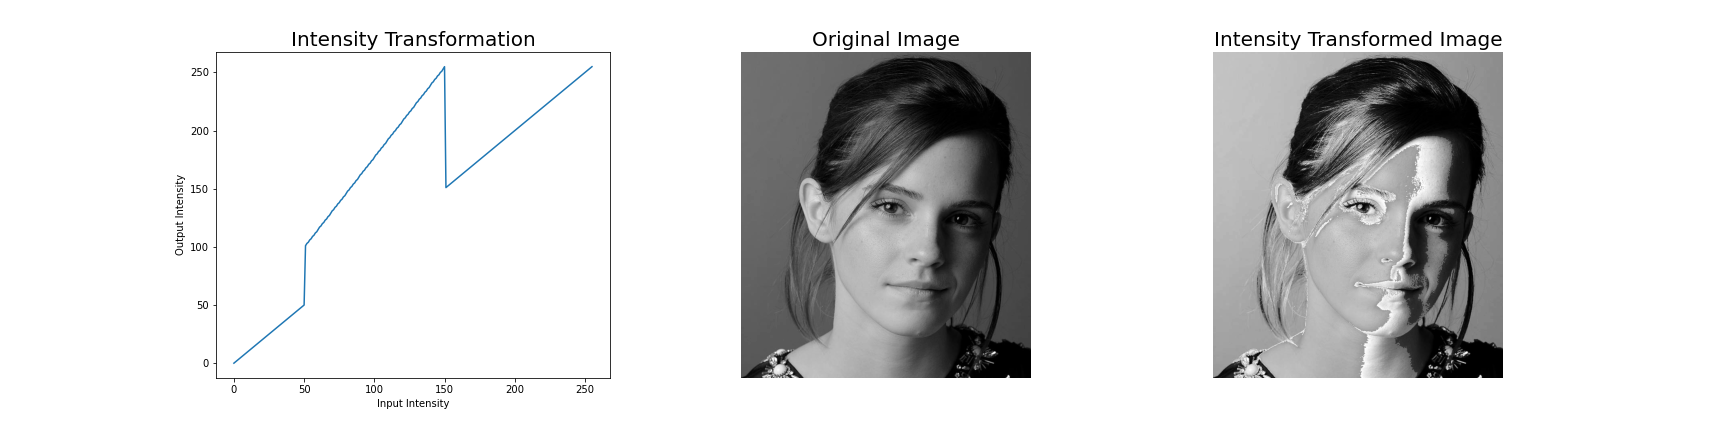
\includegraphics[width=1.25\textwidth]{../q1.png}
    \caption{Intensity Iransformation}

    \label{figq1}
\end{figure}
Figure \ref{figq1} shows the intensity transformation function,
 original image, and, the transformed image
We can see that, in this transformation function,
 pixels with intensity values between 50 and 150,
  are increased but other intensities are not changed.
   We can see this result in the above-transformed image.
    The intensities of gray pixels of the original image
     are increased so that we can see a clear white region
      on her face as well as background is also changed. But dark and white pixels are not changed.

\section*{Question 02}
To accentuate some particular pixels of an image, we can increase the
 intensity range of those pixels and reduce the intensity range of other
  pixels. i.e. increase the contrast of the required pixels. Then we can
   see more details of those pixels. Simply we can use gamma corrections
    to accentuate white and gray matter.
\subsubsection*{Accentuate White Matter}
Here I used gamma correction with $\gamma = 4$ to accentuate white matters.
\begin{lstlisting}[language=python, caption=Accentuate White Matter, label=q2c]
im = cv.imread(r"brain_proton_density_slice.png", cv.IMREAD_GRAYSCALE)
assert im is not None

white_transform = np.array([((i / 255) ** 4) * 255 for i in range(0,256)],dtype=np.uint8)
white_transformed_image = cv.LUT(im, white_transform)
    \end{lstlisting}
\begin{figure}[!htb]
    \centering
    \hspace*{-2cm}
    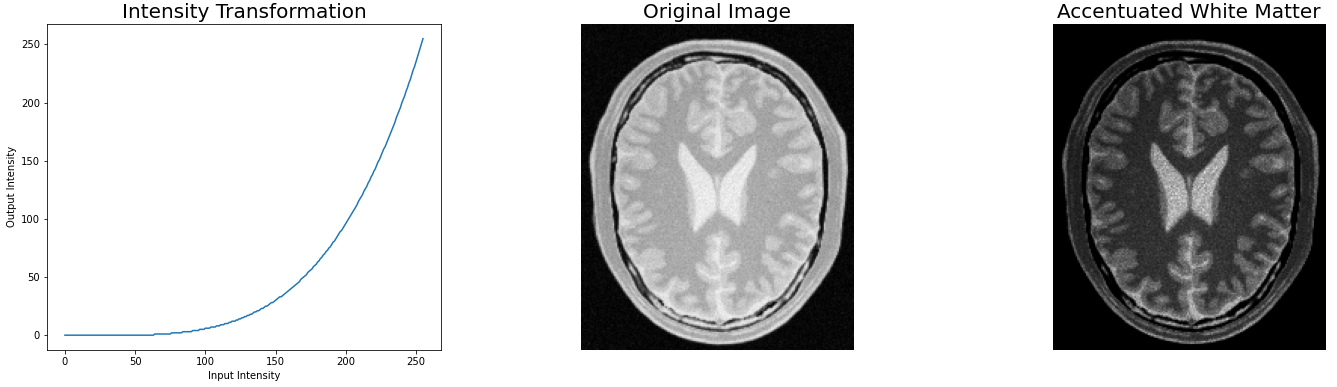
\includegraphics[width=1.2\textwidth]{../q2.png}
    \caption{Accentuate White Matter}
    \label{figq2}
\end{figure}
In this transformation, we can see that a wide range of dark pixels
 are mapped into a narrow range of dark pixels and a narrow range of
  white pixels are mapped into a wide range of white pixels. Therefore,
   we can see that the details of white matter are more highlighted
    compared to gray matter. Therefore, we can extract more information about
     white matter.
\subsubsection*{Accentuate Gray Matter}
Here I used gamma correction with $\gamma = 0.3$ to accentuate gray matters.
\begin{lstlisting}[language=python, caption=Accentuate Gray Matter, label=q22c]
gray_transform = np.array([((i / 255) ** 0.3) * 255 for i in range(0,256)],dtype=np.uint8)
gray_transformed_image = cv.LUT(im, gray_transform)
\end{lstlisting}

\begin{figure}[!htb]
    \centering
    \hspace*{-2cm}
    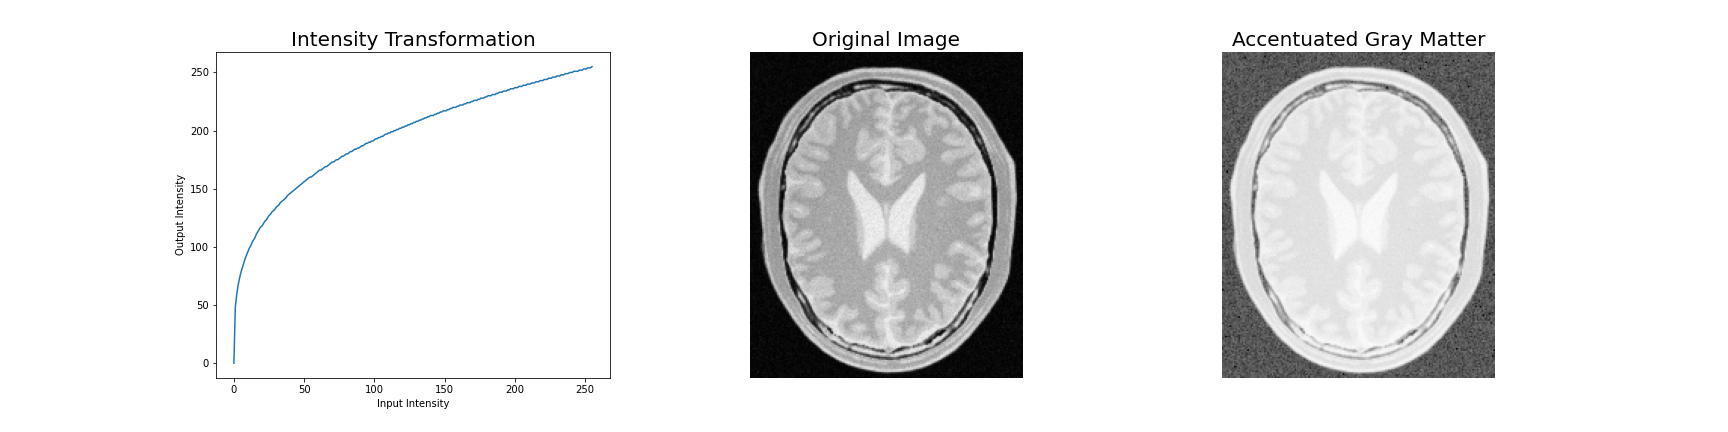
\includegraphics[width=1.2\textwidth]{../q22.png}
    \caption{Accentuate Gray Matter}
    \label{figq22}
\end{figure}

In this transformation, we can see that a narrow range of dark pixels
 are mapped into a wide range of white pixels and a wide range of white
  pixels are mapped into a narrow range of white pixels. Therefore,
   we can see that the details of gray matter are more highlighted 
   compared to white matter. Therefore, we can extract more information about
    gray matter.

\section*{Question 03}
In the L*a*b color space, L stands for Lightness. Here I applied a gamma correction with
 $\gamma = 0.4$ to the L plane.
\begin{lstlisting}[language=python, caption={Gamma Correction with $\gamma =0.4$} ]
im = cv.imread(r"highlights_and_shadows.jpg")
assert im is not None

LAB_image = cv.cvtColor(im, cv.COLOR_BGR2LAB)
original_hist = cv.calcHist([LAB_image], [0], None, [256], [0, 256])
gamma = 0.4
gamma_correction = np.array([((i / 255) ** gamma) * 255 for i in range(0,256)],dtype=np.uint8)
LAB_image[:, :, 0] = cv.LUT(LAB_image[:, :, 0], gamma_correction)

corrected_hist = cv.calcHist([LAB_image], [0], None, [256], [0, 256])
\end{lstlisting}

\begin{figure}[!htb]
    \centering
    \hspace*{-3cm}
    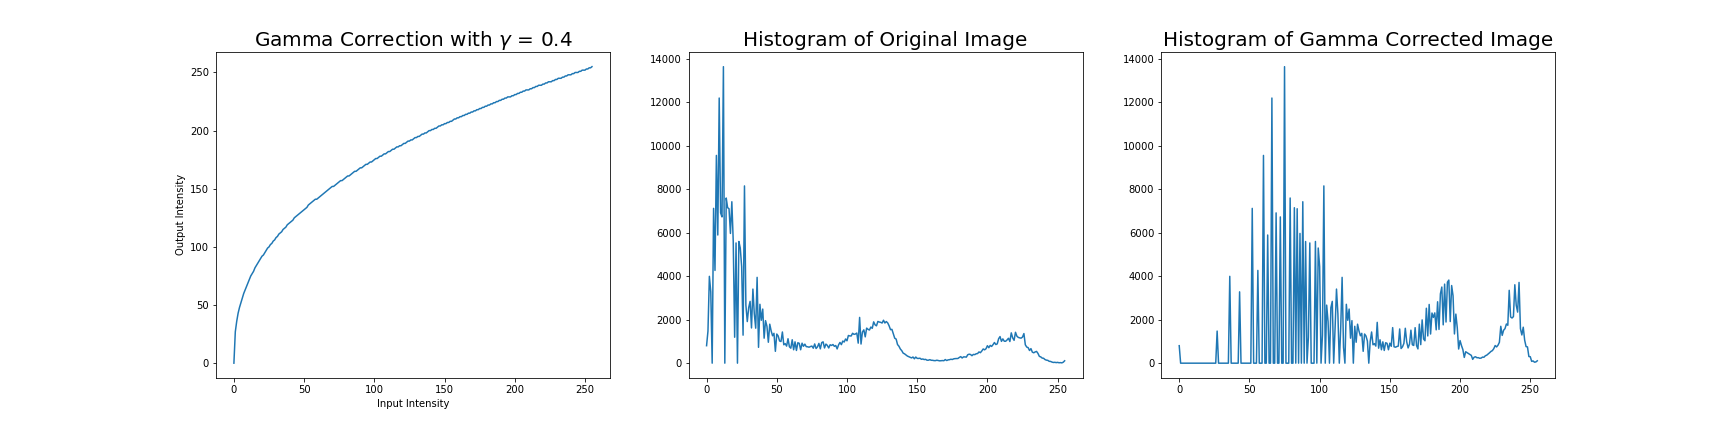
\includegraphics[width=1.3\textwidth]{../q31.png}
    \caption{}
    \label{figq31}
\end{figure}
When we apply gamma
 correction with $\gamma = 0.4$ to the L plane, the lightness of dark pixels, as well
  as light pixels, get increased.  We can see this effect on the histogram plots. In the
 original image, the histogram of the L plane is more concentrated on
  the dark region. When applying a gamma correction to the L plane, the dark pixels are shifted 
to the light region. This can be seen in the Figure \ref{figq31}.

\begin{figure}[!htb]
    \centering
    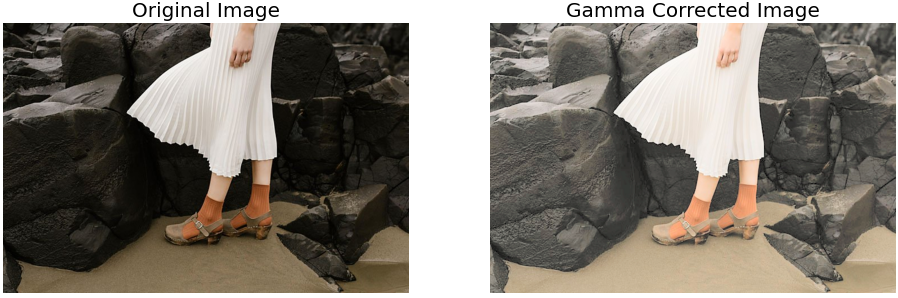
\includegraphics[width=1.1\textwidth]{../q32.png}

    \caption{Caption}
    \label{figq32}
\end{figure}

This result can be also verified from the images in Figure \ref{figq32}.
 We can see the lightness is increased in the 
Gamma corrected image compared to the Original image.

\section*{Question 04}
To perform the Histogram Equalization, first, we can get the histogram of the
 Original image using OpenCV
calcHist function. Then we can get the cumulative sum of the histogram and
 normalize it into range (0-255). Then we can perform an intensity
  transformation to the original according to normalize cumulative sum to get the
  histogram equalized image.\\

\begin{lstlisting}[language=python, caption=Histogram Equalization]
img = cv.imread(r"shells.png", cv.IMREAD_GRAYSCALE)
assert im is not None

original_hist = cv.calcHist([img], [0], None, [256], [0, 256])
cdf = original_hist.cumsum()
MN = img.shape[0] * img.shape[1]
equalize_transformation = np.array((cdf * 255) / MN, dtype=np.uint8)
equalize_img = cv.LUT(img, equalize_transformation)
equalize_hist = cv.calcHist([equalize_img], [0], None, [256], [0, 256])
\end{lstlisting}

\begin{figure}[!htb]
    \centering

    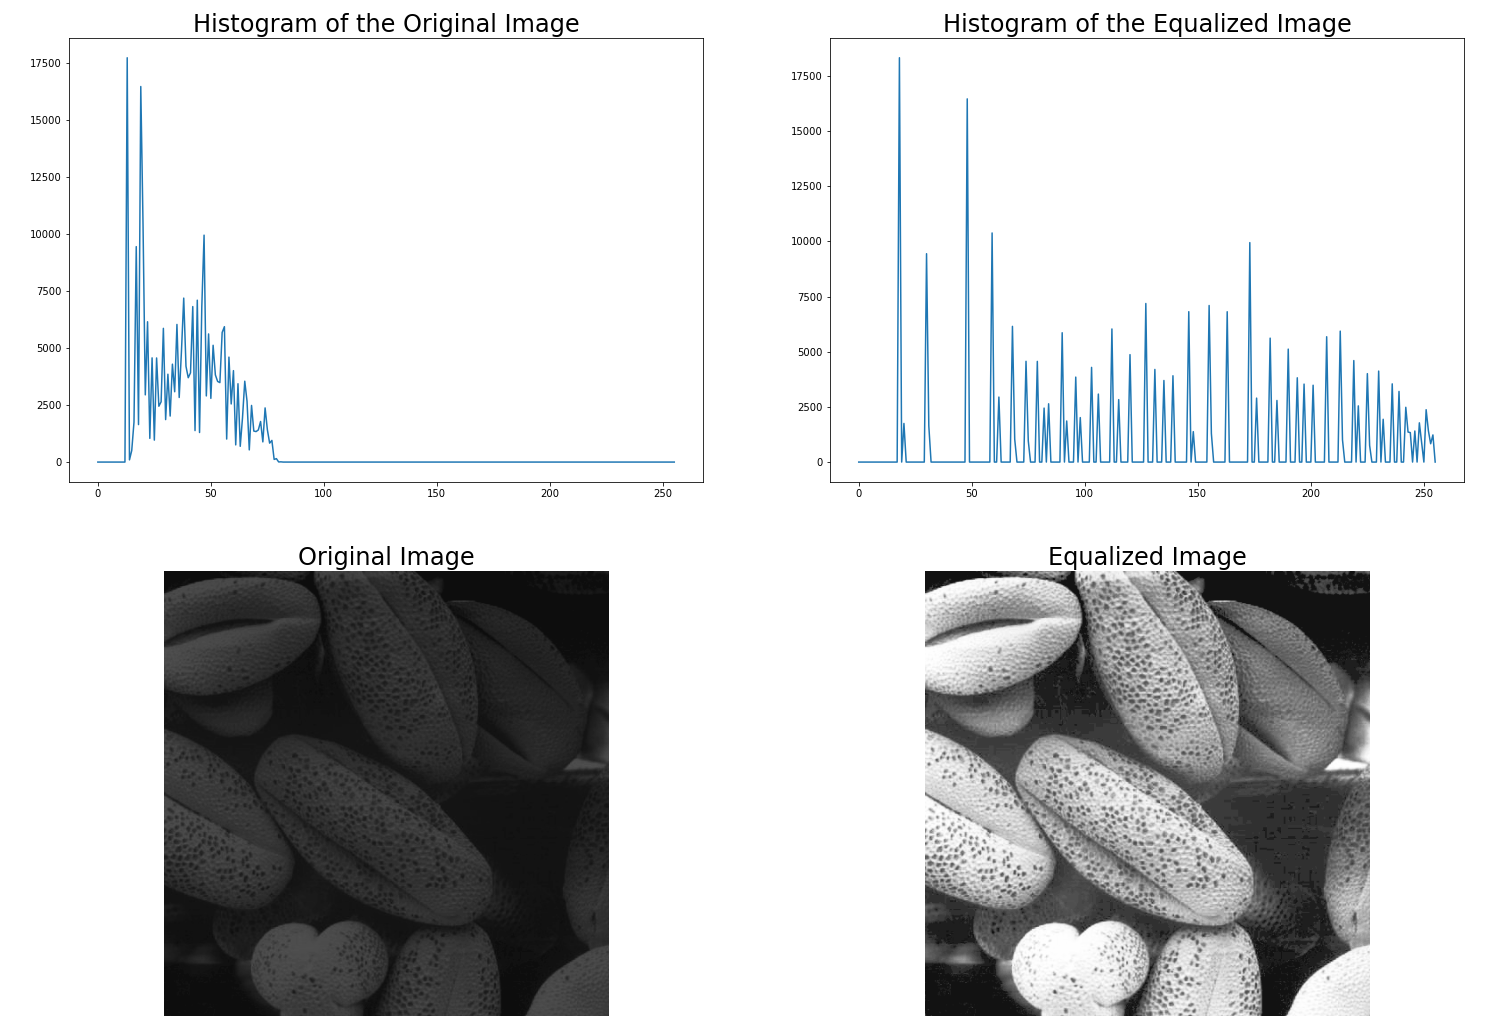
\includegraphics[width=\textwidth]{../q4.png}
    \caption{Histogram Equalization}
    \label{figq4}
\end{figure}

We can see the histogram of the original image is more concentrated on the left side. i.e. it has more dark pixels. When applying histogram equalization, we get a more spread version of the histogram. We can see this enhancement from the above images. In the original image, the contrast is very low. We cannot get any details from it. But the equalized image has more contrast. This means we can get more details/information about the original image.

\section*{Question 05}
\subsubsection*{Nearest-Neighbor Interpolation}
In the Nearest-Neighbor Interpolation, we mapped each pixel of the
 scaled image to the nearest pixel of the original image. We can do
  this by iterating each pixel of the scaled image using for loops
   and mapping each pixel value to the nearest pixel value of the original
    image.
\begin{lstlisting}[language=python, caption=Nearest-Neighbor Interpolation]
def nearestNeighborInterpolation(img, scale):
    scaled_dimentions = (round(img.shape[0] * scale), round(img.shape[1] * scale), img.shape[2])
    scaled_img = np.zeros(scaled_dimentions,dtype=np.uint8)
    for i in range(scaled_dimentions[0]):
        for j in range(scaled_dimentions[1]):
            scaled_img[i, j] = img[min(round(i / scale), img.shape[0] - 1), min(round(j / scale), img.shape[1] - 1)]
    return scaled_img
\end{lstlisting}
\subsubsection*{Bi-linear Interpolation}
In the Bilinear Interpolation, we mapped each pixel of the scaled
 image to the original image by linear interpolating along the
  x-axis and y-axis.

\begin{lstlisting}[language=python, caption=Bi-linear Interpolation]
def bilinearInterpolation(img, scale):
    scaled_dimentions = (round(img.shape[0] * scale), round(img.shape[1] * scale), img.shape[2])
    scaled_img = np.zeros(scaled_dimentions,dtype=np.uint8)
    y_ratio = (img.shape[1] - 1) / (scaled_dimentions[1] - 1)
    x_ratio = (img.shape[0] - 1) / (scaled_dimentions[0] - 1)
    for i in range(scaled_dimentions[0]):
        for j in range(scaled_dimentions[1]):
            y_floor = math.floor(j * y_ratio)
            y_ceil = min(math.ceil(j * y_ratio), img.shape[1] - 1)
            x_floor = math.floor(i * x_ratio)
            x_ceil = min(math.ceil(i * x_ratio), img.shape[0] - 1)
            y_weight = (j * y_ratio) - y_floor
            x_weight = (i * x_ratio) - x_floor
            pixel_value = img[x_floor, y_floor] * (1 - y_weight) * (1 - x_weight) + \
                img[x_ceil, y_floor] * (1 - y_weight) * (x_weight) + \
                    img[x_floor, y_ceil] * (y_weight) * (1 - x_weight) + \
                        img[x_ceil, y_ceil] * (y_weight) * (x_weight)
            
            scaled_img[i, j] = pixel_value
            
    return scaled_img
\end{lstlisting}

\begin{figure}[!htb]
    \centering
    %\hspace*{-2cm}
    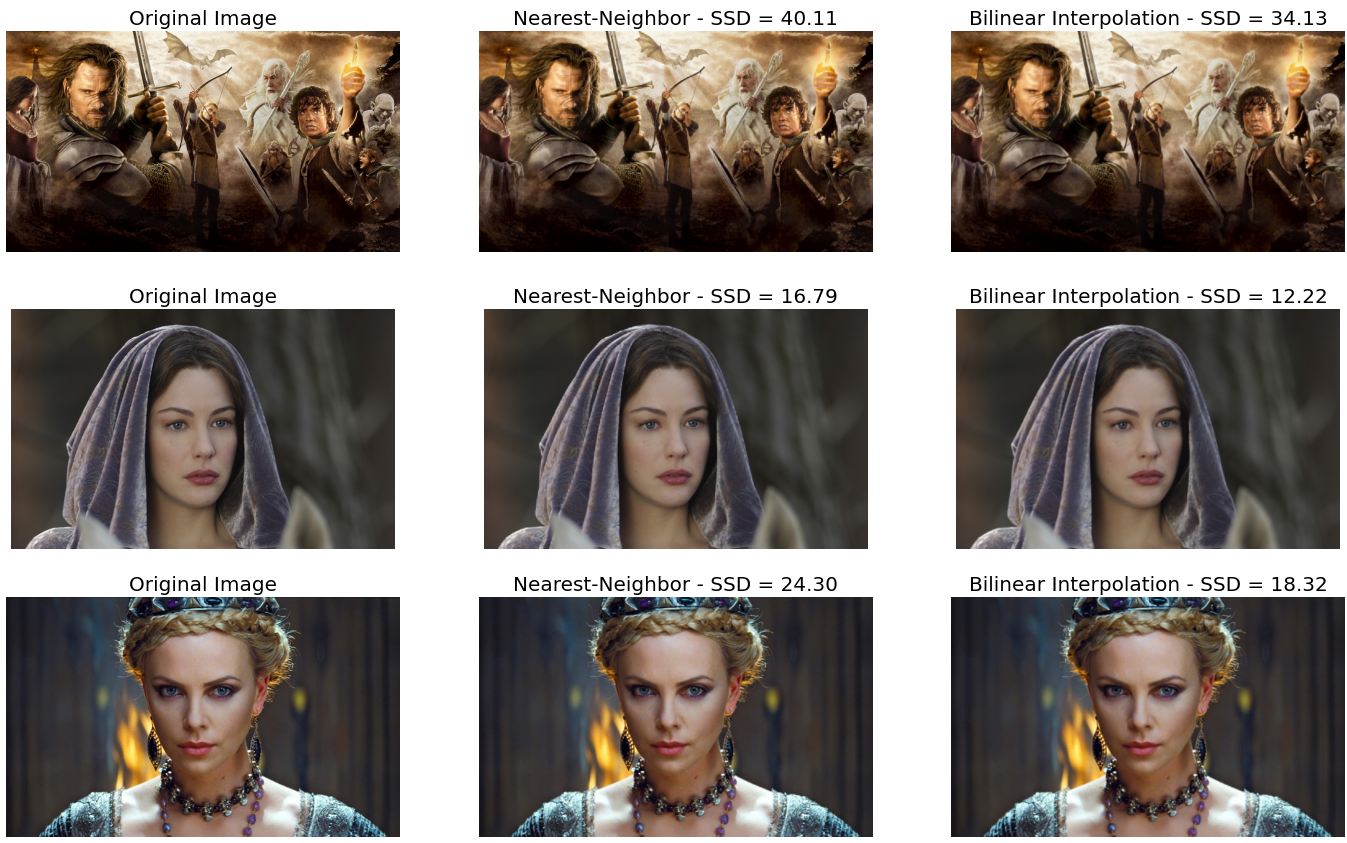
\includegraphics[width=\textwidth]{../q5.png}
    \caption{Comparison of Zooming}
    \label{figq5}
\end{figure}
In the Nearest-Neighbor Interpolation, if we inspect closely, we
 can see there are small square-shaped fragments in the zoomed image. This happens
  because in this method we just approximate the pixel values to
   their nearest pixel value in the original image. Therefore we
    can see the same pixel is appearing in small square-shaped regions.
     But in the Bilinear Interpolation, we don’t see this kind of behavior
      This is because, in this method, we approximate the pixel value
       by averaging it along the x-axis and y-axis. Therefore, we
        can see a smooth image when applying Bilinear Interpolation.
        Therefore, we can say that Bilinear Interpolation performs better
         than Nearest-Neighbor Interpolation. This can be also verified
          quantitatively using the below method.

We can get a quantitative idea of the quality of these two interpolations,
 by calculating the Normalized Sum of Squared Difference (SSD) of two
  resultant images. Listing \ref{ssd} shows the snipped code of the SSD
   function.
\begin{lstlisting}[language=python, caption=SSD, label=ssd]
def SSD(img1, img2):
    return (np.power((img1 - img2), 2)).sum() / (img1.size)
\end{lstlisting}
The SSD value is shown at the top of each image. We can observe that
 in each 3 cases, Bilinear Interpolation gives a low SSD value compared
  to Nearest-Neighbor Interpolation. This means Bilinear Interpolation
   approximates the original image better than Nearest-Neighbor
    Interpolation.



\section*{Question 06}
\subsubsection*{Using filter2D}
Sobel filtering can be used to get the edges of an image. Sobel
 vertical kernel extracts the horizontal edges and Sobel horizontal
  kernel extracts the vertical edges. I this part OpenCV filter2D
   function is used to apply the kernel.
\begin{lstlisting}[language=python]
img = cv.imread(r"einstein.png", cv.IMREAD_GRAYSCALE).astype(np.float32)
assert im is not None

sobel_v_kernel = np.array([[-1, -2, -1], [0, 0, 0], [1, 2, 1]], dtype=np.float32)
f_x = cv.filter2D(img, -1, sobel_v_kernel)
sobel_h_kernel = np.array([[-1, 0, 1], [-2, 0, 2], [-1, 0, 1]], dtype=np.float32)
f_y = cv.filter2D(img, -1, sobel_h_kernel)
grad_mag_img = np.sqrt(f_x**2 + f_y**2)
\end{lstlisting}
\begin{figure}[!htb]
    \centering
    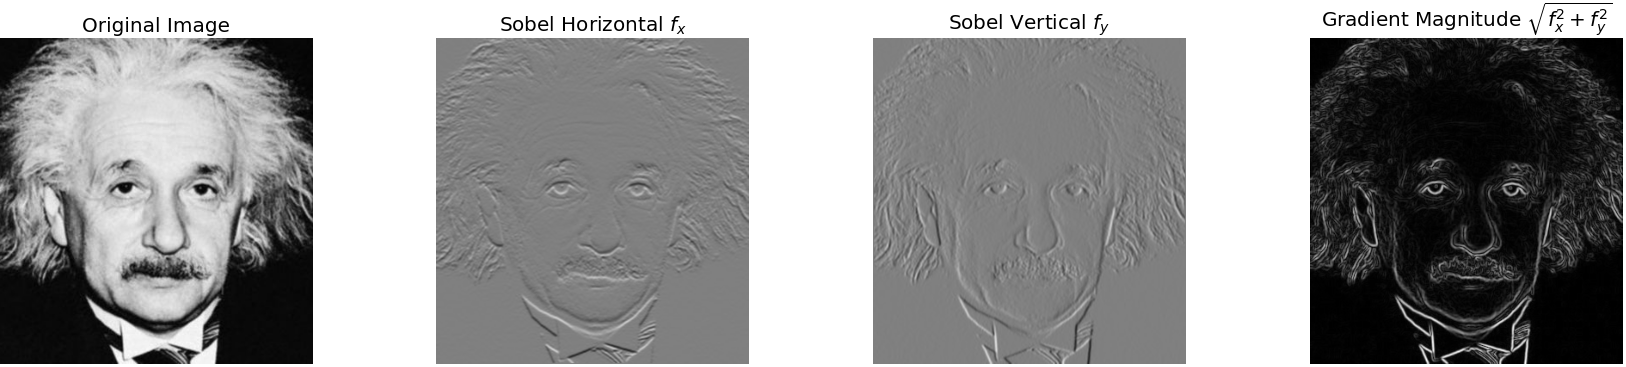
\includegraphics[width=\textwidth]{../q61.png}
    \caption{Using filter2D}
    \label{fig61}
\end{figure}

\subsubsection*{Using Manually Coded Filter Function}
This function takes the image and the kernel as the parameters.
 First, it rotates the kernel 180 to perform the convolution operation.
  Then adds the padding zeros to the boundaries of the image according
   to the given kernel size. After that, it applies the kernel to the
    image using 2 for loops.
\begin{lstlisting}[language=python]
def spacial_filter(img, kernel):
    assert kernel.shape[0]%2 == 1 and kernel.shape[1]%2 == 1
    kernel = np.rot90(np.rot90(kernel)) # rotate 180 for convolution
    v_padding = int(kernel.shape[0] / 2)
    h_padding = int(kernel.shape[1] / 2)
    padded_img = np.zeros((img.shape[0] + 2 * v_padding, img.shape[1] + 2 * h_padding ), dtype=np.float32)
    padded_img[v_padding:padded_img.shape[0] - v_padding, h_padding:padded_img.shape[1] - h_padding] = img
    filtered_image = np.zeros(img.shape, dtype=np.float32)
    for i in range(filtered_image.shape[0]):
        for j in range(filtered_image.shape[1]):
            filtered_image[i, j] = (kernel * padded_img[i: i + kernel.shape[0], j: j + kernel.shape[1]]).sum()
    return filtered_image

f_x = spacial_filter(img, np.array([[-1, -2, -1], [0, 0, 0], [1, 2, 1]], dtype=np.float32))
f_y = spacial_filter(img, np.array([[-1, 0, 1], [-2, 0, 2], [-1, 0, 1]], dtype=np.float32))
grad_mag_img = np.sqrt(f_x**2 + f_y**2)
\end{lstlisting}
\begin{figure}[!htb]
    \centering
    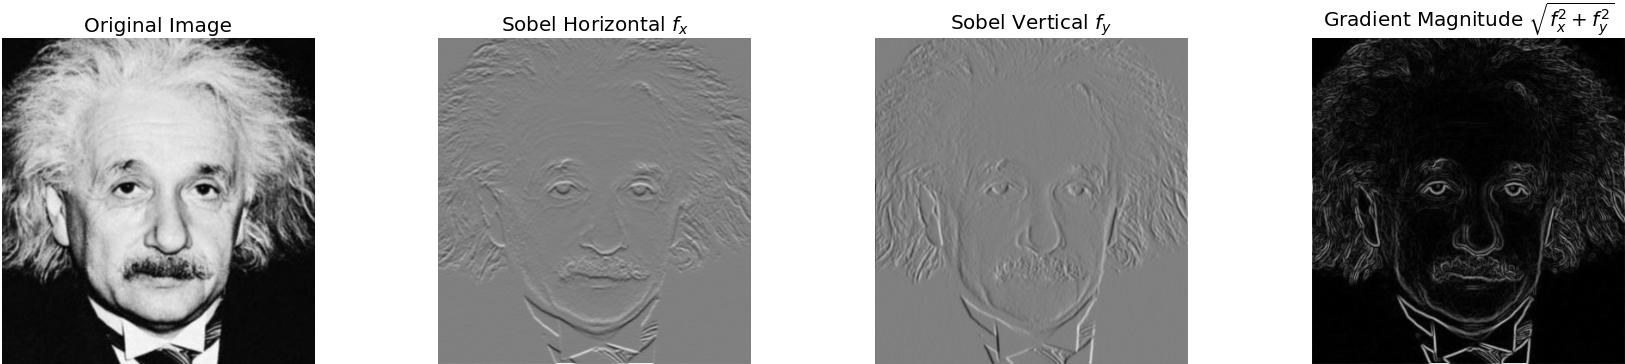
\includegraphics[width=\textwidth]{../q62.png}
    \caption{Using Manually Coded Filter Function}
    \label{figq62}
\end{figure}

\subsubsection*{Using the Outer Product Property}
We use the outer product property to perform the Sobel filtering
 (This can be also referred to as convolution of row vector and
  column vector). First, we apply the vertical kernel to the
   image and then apply the horizontal kernel to the resulting
    image. Here I used the special\_filter function created
     by me, to apply the filter. We can also use the OpenCV
      filter2D function twice or the sepFilter2D function to
       apply the vertical kernel and horizontal kernel. This
        method is more efficient than the previous method
         because applying row kernel or column kernel needs 
         fewer computations.
\begin{lstlisting}[language=python]
f_y = spacial_filter(img, np.array([[1], [2], [1]], dtype=np.float32))
f_y = spacial_filter(f_y, np.array([[1, 0, -1]], dtype=np.float32))

f_x = spacial_filter(img, np.array([[1], [0], [-1]], dtype=np.float32))
f_x = spacial_filter(f_x, np.array([[1, 2, 1]], dtype=np.float32))
grad_mag_img = np.sqrt(f_x**2 + f_y**2)
\end{lstlisting}
\begin{figure}[!htb]
    \centering
    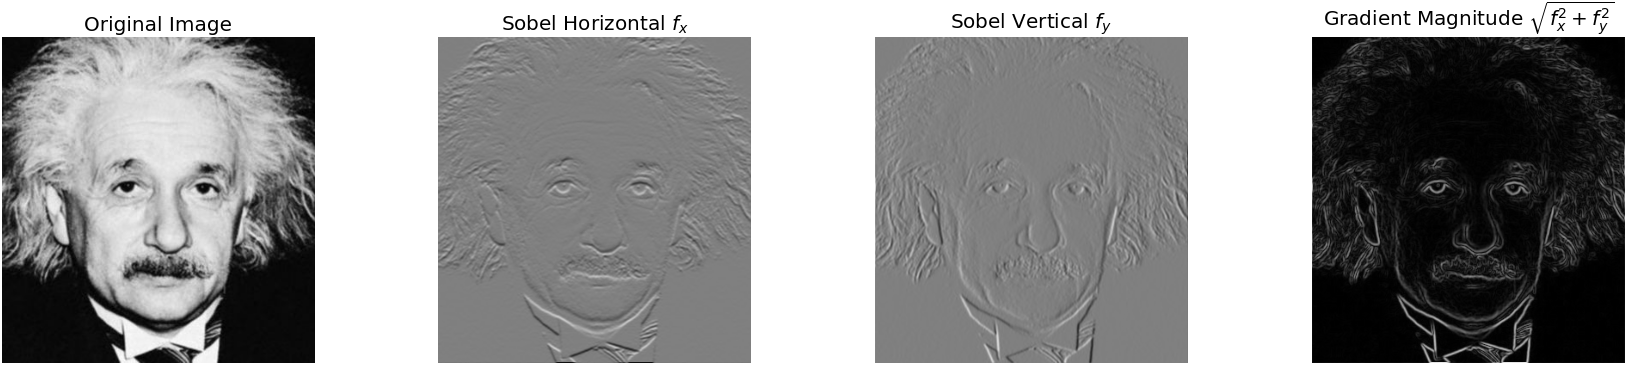
\includegraphics[width=\textwidth]{../q63.png}
    \caption{Using the Outer Product Property}
    \label{figq63}
\end{figure}
Each 3 methods describe above gives the same results. We
 can see that Sobel horizontal filter extracts vertical edges
  of the face and Sobel vertical filter extracts horizontal
   edges of the face. The Gradient magnitude is calculated by
    squaring the Sobel vertical image and horizontal image and
     taking the square root. Therefore, it has vertical edges as
      well as horizontal edges. Therefore, we can see all the
       edges of the face in the gradient magnitude image.

\section*{Question 07}
\begin{lstlisting}[language=python]
img = cv.imread(r"daisy.jpg")
assert im is not None

rect = (51,147,507,441)
mask = np.zeros(img.shape[:2], dtype=np.uint8)
x,y,w,h = rect
mask[y:y+h, x:x+w] = 1 

fgModel = np.zeros((1, 65), dtype="float")
bgModel = np.zeros((1, 65), dtype="float")
cv.grabCut(img, mask, rect, bgModel,fgModel,iterCount=10, mode=cv.GC_INIT_WITH_RECT)
mask2 = np.where((mask==2)|(mask==0),0,1).astype(np.uint8)
foreground_img = img*mask2[:, :, np.newaxis] 
background_img = img*(1 - mask2[:, :, np.newaxis])
\end{lstlisting}
\begin{figure}[!htb]
    \centering
    \hspace*{-1cm}
    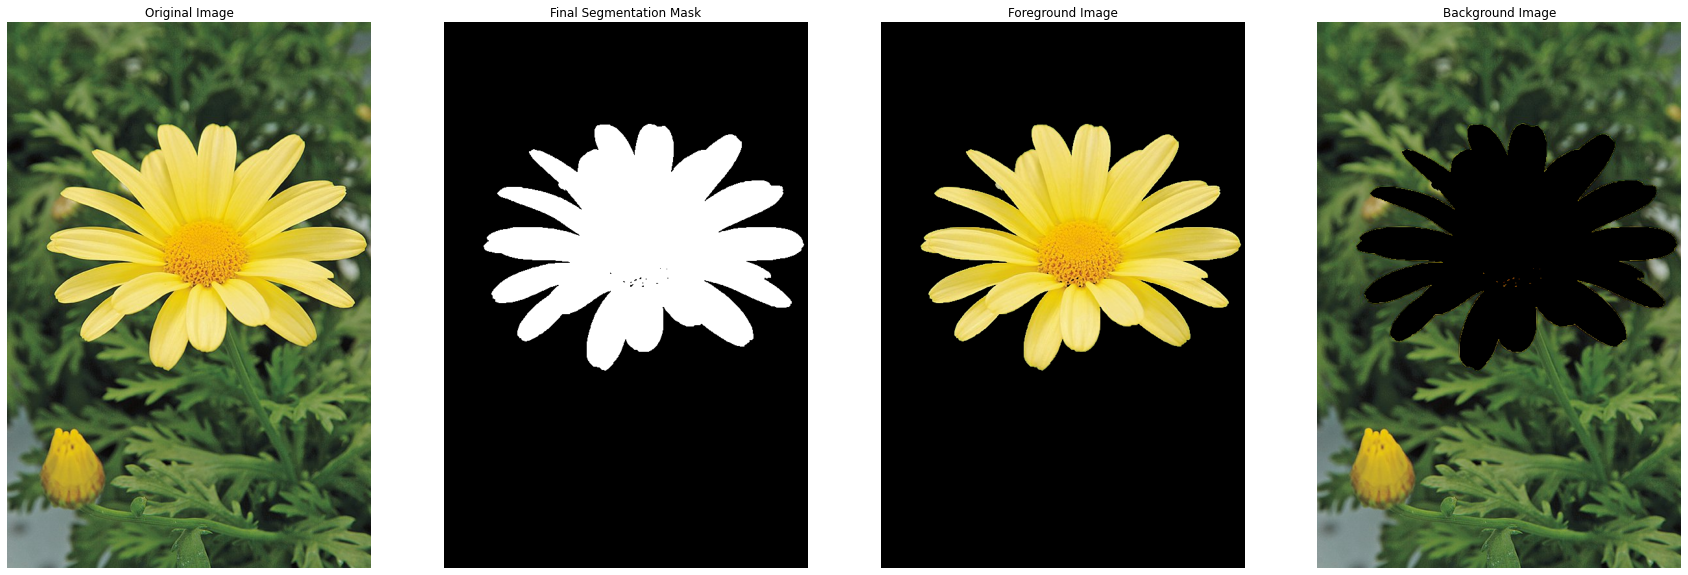
\includegraphics[width=1.1\textwidth]{../q7.png}
    \caption{Caption}
    \label{fig:my_label}
\end{figure}

\begin{lstlisting}[language=python]
background_blurred_img = cv.GaussianBlur(background_img, (13, 13), 8)
enhanced_img = foreground_img + background_blurred_img*(1 - mask2[:, :, np.newaxis])
\end{lstlisting}

\end{document}
